\chapter{Malware}

\section{Rede}

Nesta sección trataranse as implicacións de seguridade que poidan ter as diferentes tecnoloxías de contedorización segundo o seu modelo de rede.

\subsection{Docker}

O modelo de rede de Docker está composto por un subsistema de rede virtual que permite finalmente aos diferentes contedores conectarse á rede que emprega a máquina anfitrioa.\\

Tal e como vén reflectido na documentación oficial de Docker \cite{docker-networking}, non existe unha única forma de despregar este subsistema de rede, senón que coexisten diversos modelos que podemos escoller baixo libre elección: \textit{bridge, host, overlay, macvlan} ou \textit{none}. Cada un deles pensado para seres empregado en diferentes casos de uso.\\

Analizaremos con detemento o modo \textit{bridge}, posto que é o modo por defecto no que o subsistema de rede de Docker é despregado, ademais de ser o modo recomendado para executar contedores independentes que se precisan comunicar. É dicir, cando iniciamos Docker, unha rede \textit{bridge} é creada automaticamente, e será empregada por defecto polos novos contedores \cite{docker-bridge-networks}. Este modo de execución é o máis común, xa que normalmente non interesa executar un contedor illado, senón que se poida comunicar co exterior.\\

Se continuamos lendo un pouco máis sobre o funcionamento deste modo de rede, podemos atopar na sección de seguridade da documentación oficial de Docker que dende un punto de vista arquitectónico, todos os contedores conectados en rede nun anfitrión Docker mediante unha interface \textit{bridge} son equivalentes a máquinas físicas conectadas mediante un \textit{switch Ethernet} común; nin máis, nin menos \cite{docker-security}.\\

Por tanto, cando se crea un novo contedor Docker, tamén se establece unha nova interface virtual \textit{Ethernet} cun nome único e se conecta ao nomeado \textit{bridge} ou ponte de rede. Esta interface estará conectada ao interface de rede \textit{eth0} do contedor, permitindo así mandar paquetes á ponte dende o mesmo. Este modelo de conectividade establecido por defecto por Docker é susceptíbel a ataques como \textit{ARP spoofing} ou \textit{Mac flooding}, posto que a ponte permite o reenvío (\textit{forwarding}) de todos os paquetes recibidos sen ningún tipo de filtrado \cite{Securing-Docker-Containers-from-Denial-of-Service}.\\

Detectado, por tanto, un posíbel vector de ataque, por mor da estrutura de rede seguida por Docker, cómpre realizar probas que aseguren dito comportamento.

%Indicar que os contedores Docker correron no Cloud Open Nebula do CESGA, por riba dunha MV

\subsubsection{Probas}

Para poderes comprobar que as vulnerabilidades previamente estudadas son realmente un posíbel vector de ataque na emprega de contedores Docker, creouse unha pequena estrutura de contedores coa axuda de Docker Compose, tal e como ven especificado no anexo \ref{codigo-arp-spoofing}, conectando en rede aos mesmos. A estrutura creada está composta por:

\begin{itemize}
    \item Un contedor servidor correndo Nginx 1.13.10.
    \item Un contedor cliente correndo Ubuntu Xenial 16.04.
    \item Un contedor atacante correndo Kali Linux 2018.1.
\end{itemize}

Devandita estrutura foi levantada sobre unha máquina virtual Ubuntu Xenial 16.04 aloxada no Cloud Open Nebula do CESGA. A composición final pode ser apreciada na figura \ref{DiagramaRedeDockerCloud}.\\

\begin{figure}
\centerline{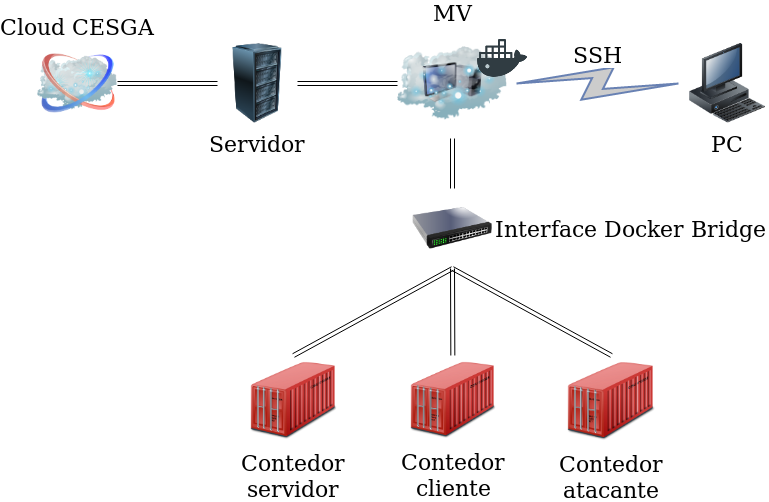
\includegraphics[width=15cm]{figuras/DiagramaRedeDockerCloud.png}}
\caption{Diagrama de Rede Docker Cloud}
\label{DiagramaRedeDockerCloud}
\end{figure}

Aproveitando as debilidades da rede asociadas ao modelo establecido nos contedores Docker, tratarase de obter tráfico da rede de forma ilexítima dende o contedor atacante namentres se realiza unha comunicación entre os contedores cliente e servidor.

\paragraph{\textit{ARP spoofing}}~~

%TODO citar to docker or not to docker: El único defecto es que todos los contenedores comparten el mismo puente de red, lo que permite ataques de envenenamiento con el protocolo de resolución de direcciones (ARP) entre contenedores en el mismo host. ---> Namespace isolation and capabilities drop are enabled by default, but cgroups limitations aren’t; they must be enabled on a per-container basis through -a -c options on container launch. The default isolation configuration is relatively strict. The only flaw is that all containers share the same network bridge, enabling Address Resolution Protocol (ARP) poisoning attacks between containers on the same host

Para comprender o que se pretende facer con este ataque, é importante explicar primeiramente de que se trata.\\

O protocolo ARP (\textit{Address Resolution Protocol} ou Protocolo de Resolución de Direccións) é un dos protocolos de rede máis básicos pero máis esenciais que existen. É o encargado de resolver a dirección física (MAC) dunha máquina dada a súa dirección IP. O seu funcionamento baséase no envío dun paquete, \textit{ARP request}, a todos os integrantes da rede (\textit{broadcast}) que contén a IP pola que se pregunta e agárdase a que a máquina asociada a devandita IP responda (ARP \textit{reply}) coa súa dirección física correspondente. Cada máquina manterá unha caché coas direccións traducidas para reducir o retardo, conformando así a denominada táboa ARP. Polo tanto, o protocolo ARP permite a independencia das direccións IP e MAC.\\

Por mor da apátrida do protocolo e da falta de mecanismos de autenticación para verificar a identidade do remitente, o protocolo ARP ten unha longa historia de propensión como vector de ataques de suplantación \cite{detectingARPSpoofing}. Así, intrinsecamente asociado ao funcionamento deste protocolo existe o risco de suplantación de ARP, ou \textit{ARP spoofing}. Este consiste no envío de mensaxes ARP falsas á \textit{Ethernet}, obtendo así asociar a dirección MAC do atacante coa dirección IP doutra máquina (a vítima). Como consecuencia deste feito, calquera tráfico dirixido a esa dirección IP será erroneamente enviado ao atacante, no canto de acadar o seu destino lexítimo.\\

Chegados a este punto, o atacante pode levar a cabo diversas accións:

\begin{itemize}
\item Reenviar os paquetes ao seu verdadeiro destinatario, producíndose un ataque \textit{Man-in-the-middle} (MITM), no que ademais pode:
    \begin{itemize}
    \item Reenviar os paquetes sen modificar o seu contido.
    \item Modificar o contido dos paquetes e logo reenvialos ao destinatario.
    \end{itemize}
\item Asociar unha dirección MAC inexistente coa dirección IP da porta de enlace predeterminada da vítima, evitando así a comunicación da misma co exterior e producíndose por tanto un ataque de denegación de servizo (DoS).
\end{itemize}

A suplantación ARP supón en moitas ocasións o punto de partida para ataques de rede máis sofisticados, como ataques de denegación de servizo, \textit{Man in the middle} ou secuestro de sesións.\\

Posto que o risco existe polo simple xeito de conectar unha máquina á rede local mediante \textit{Ethernet}, o modelo de rede de Docker previamente explicado fai que sexa susceptíbel de por si ao ataque. Realizarase unha proba baixo a estrutura da figura \ref{DiagramaRedeDockerCloud} para confirmalo. Os pasos seguidos foron os seguintes:

\begin{enumerate}
\item Previo ao ataque:

En primeira instancia compróbanse todas as direccións IP e físicas, así como as táboas ARP dos contedores cliente e servidor.

\begin{lstlisting}[,caption={Consulta direccións IP e física no contedor atacante}]
root@9f3f255ace4a:/# ifconfig 
eth0: flags=4163<UP,BROADCAST,RUNNING,MULTICAST>  mtu 1500
        inet 172.18.0.4  netmask 255.255.0.0  broadcast 0.0.0.0
        inet6 fe80::42:acff:fe12:4  prefixlen 64  scopeid 0x20<link>
        ether 02:42:ac:12:00:04  txqueuelen 0  (Ethernet)
        RX packets 36822  bytes 82108747 (78.3 MiB)
        RX errors 0  dropped 0  overruns 0  frame 0
        TX packets 36389  bytes 2895807 (2.7 MiB)
        TX errors 0  dropped 0 overruns 0  carrier 0  collisions 0
\end{lstlisting}

\begin{lstlisting}[,caption={Consulta direccións IP e física no contedor cliente}]
root@20136c4451bb:/# ifconfig 
eth0      Link encap:Ethernet  HWaddr 02:42:ac:12:00:02  
          inet addr:172.18.0.2  Bcast:0.0.0.0  Mask:255.255.0.0
          inet6 addr: fe80::42:acff:fe12:2/64 Scope:Link
          UP BROADCAST RUNNING MULTICAST  MTU:1500  Metric:1
          RX packets:5527 errors:0 dropped:0 overruns:0 frame:0
          TX packets:1708 errors:0 dropped:0 overruns:0 carrier:0
          collisions:0 txqueuelen:0 
          RX bytes:30975137 (30.9 MB)  TX bytes:124933 (124.9 KB)
\end{lstlisting}

\begin{lstlisting}[,caption={Consulta direccións IP e física no contedor servidor}]
root@07cecfe068f2:/# ifconfig 
eth0: flags=4163<UP,BROADCAST,RUNNING,MULTICAST>  mtu 1500
        inet 172.18.0.3  netmask 255.255.0.0  broadcast 0.0.0.0
        inet6 fe80::42:acff:fe12:3  prefixlen 64  scopeid 0x20<link>
        ether 02:42:ac:12:00:03  txqueuelen 0  (Ethernet)
        RX packets 3848  bytes 10735169 (10.2 MiB)
        RX errors 0  dropped 0  overruns 0  frame 0
        TX packets 1291  bytes 92650 (90.4 KiB)
        TX errors 0  dropped 0 overruns 0  carrier 0  collisions 0
\end{lstlisting}

Polo tanto:

\begin{table}[H]
\centering
\caption{Direccións de rede dos contedores}
\label{direccions-rede}
\begin{tabular}{|c|c|c|}
\hline
Contedor & Dirección IP & Dirección física \\ \hline
Atacante & 172.18.0.4 & 02:42:ac:12:00:04 \\ \hline
Cliente & 172.18.0.2 & 02:42:ac:12:00:02 \\ \hline
Servidor & 172.18.0.3 & 02:42:ac:12:00:03 \\ \hline
\end{tabular}
\end{table}

\item Execución do ataque:

Para executar o ataque, o contedor atacante enviará en bucle numerosas mensaxes ARP aos contedores cliente e servidor, co fin de envelenar as súas respectivas táboas ARP e tendo lugar por conseguinte un ataque MITM. Para elo, empregarase o \textit{software} \textit{arpspoof}, pertencente ao paquete de utilidades \textit{dsniff}\footnote{https://www.monkey.org/~dugsong/dsniff/}.

\begin{lstlisting}[,caption={Envelenamento táboas ARP dende contedor atacante}]
root@9f3f255ace4a:/# arpspoof -i eth0 172.18.0.2 -t 172.18.0.3 &
root@9f3f255ace4a:/# arpspoof -i eth0 172.18.0.3 -t 172.18.0.2 &
\end{lstlisting}

\item Comprobación do ataque:

Unha vez foron enviadas algunhas mensaxes ARP co fin de envelenar as táboas dos contedores cliente e servidor, comprobaremos que o ataque efectuouse correctamente. Para iso, inspeccionáronse novamente as táboas ARP, onde agora pódese ver con total claridade que as asociacións entre direccións físicas e IP víronse truncadas, facendo chegar por tanto paquetes non lexítimos ao contedor atacante. Ademais, no contedor atacante executaremos a utilidade \textit{urlsnarf}, pertencente tamén ao paquete \textit{dsniff}, o cal mostrará por pantalla todas as URLs solicitadas, como forma de comprobar o éxito do ataque MITM. No proceso será necesario que, por exemplo, o contedor cliente solicite unha páxina web ao contedor servidor.

\begin{lstlisting}[,caption={Consulta táboa ARP do contedor cliente}]
root@20136c4451bb:/# arp -a
arpspoof_kali_1.arpspoof_default (172.18.0.4) at 02:42:ac:12:00:04 [ether] on eth0
? (172.18.0.1) at 02:42:39:9e:31:24 [ether] on eth0
arpspoof_nginx_1.arpspoof_default (172.18.0.3) at 02:42:ac:12:00:04 [ether] on eth0
\end{lstlisting}

\begin{lstlisting}[,caption={Consulta táboa ARP do contedor servidor}]
root@07cecfe068f2:/# arp -a
arpspoof_kali_1.arpspoof_default (172.18.0.4) at 02:42:ac:12:00:04 [ether] on eth0
? (172.18.0.1) at 02:42:39:9e:31:24 [ether] on eth0
arpspoof_ubuntu_1.arpspoof_default (172.18.0.2) at 02:42:ac:12:00:04 [ether] on eth0
\end{lstlisting}

\begin{lstlisting}[,caption={Solicitude páxina web dende o contedor cliente ao contedor servidor}]
root@20136c4451bb:/# curl nginx
<!DOCTYPE html>
<html>
.
.
.
</html>
\end{lstlisting}

\begin{lstlisting}[,caption={Escoita de solicitudes web con \textit{urlsnarf} dende o contedor atacante}]
root@9f3f255ace4a:/# urlsnarf -i eth0
urlsnarf: listening on eth0 [tcp port 80 or port 8080 or port 3128]

arpspoof_ubuntu_1.arpspoof_default - - [06/Apr/2018:08:57:08 +0000] "GET http://nginx/ HTTP/1.1" - - "-" "curl/7.47.0"
\end{lstlisting}

Por tanto, queda demostrado que o envelenamento efectuouse con éxito e que o contedor atacante é quen de escoitar as conexión que se realizan entre os outros contedores (MITM), o cal ten serias consecuencias, como modificar o contido dos paquetes intercambiados se así quixer, ou efectuar un ataque de denegación de servizo.

\end{enumerate}

\subsection{Singularity}

%Indicar aquí o modelado de rede de Singularity.

Singulatity emprega a mesma rede que calquera outro proceso da máquina anfitrioa. Posto que Singularity non emula nengún paradigma de virtualización a nivel de hardware, non é necesario separr as redes do espacio illado dos contedores do resto do sistema, xa que, en principio, non existe o concepto de escalada de privilexios dentro dos contedores Singularity. É dicir, os programas executados baixo un contedor Singularity terá os mesmos privilexios que se o fixera dende fóra, polo que o risco de controlar a rede non dependerá da emprega de contedores. \cite{SingularityHPC} \\

Grazas a este modelo de rede, Singularity non pode ser vulnerábel aos ataques aos que Docker, por defecto, sí que o é, posto que comparte a rede coa da propia máquina anfitrioa e os permisos dentro do contedor son os mesmos que fóra del.\\

Un posíbel vector de ataque viría dado pola escalada de privilexios e tentar executar programas de rede con permisos de superusuario dentro do contedor. Este feito será estudado con máis detalle na sección \ref{demo-fail-escalada}.

\section{Límites de recursos}

A limitación dos recursos físicos é unha cuestión moi importante no referente á seguridade do sistema, xa que un contedor malicioso podería facer uso exhaustivo dos mesmos, chegando a ocupar a práctica totalidade destes e perxudicando así a outros contedores aloxados na mesma máquina, ou mesmamente á propia máquina anfitrioa, podéndose producir así un ataque de deneganición de servizo (DOS) \cite{OS-level-security}. Numerosos aspectos deben ser tidos en conta para asegurar a seguridade integral do sistema no referente á utilización adecuada dos recursos físicos. Dividiremos por tanto o estudo en: CPU, memoria, disco e rede.\\

Analizaremos as diferentes respostas a este tipo de sobreutilizacións de recursos, tentando facer unha comparativa entre execucións debidamente controladas e outras que non o estarán, para o cal empregaranse pequenas aplicacións contedorizadas.

\subsection{Docker}

Docker relega algunha das súas funcionalidades de seguridade directamente nas inherentes características do \textit{kernel} de GNU/Linux. Polo tanto, o límite dos privilexios entre os contedores e a máquina anfitrioa xa foi deseñado. Os controis técnicos que levan este límite inclúen o illamento de procesos mediante os espazos de nomes (\textit{namespaces}\footnote{http://man7.org/linux/man-pages/man7/namespaces.7.html}), permitindo así illar usuarios, procesos, redes ou dispositivos, e administración dos recursos mediante \textit{cgroups}\footnote{http://man7.org/linux/man-pages/man7/cgroups.7.html}.\\

Deste xeito, os contedores Docker execútanse baixo un suposto entorno illado e controlado na máquina anfitrioa. Este illamento lógrase mediante os xa nomeados controis, espazos de nomes e \textit{cgroups}, que se fusionaron a partir da versión 2.6.24 do \textit{kernel} de GNU/Linux. No referente aos límites de recursos, debemos pór a nosa atención nos \textit{cgroups}, posto que o seu obxectivo é precisamente que un proceso non tome todos os recursos dispoñíbeis do sistema. Isto inclúe os recursos partillados de CPU, memoria, ancho de banda da rede e E/S de disco \cite{To-Docker-Or-Not-To-Docker}. \\

Debido a estas delegacións de seguridade sobre os \textit{cgroups}, non debemos influir na súa funcionalidade (e polo tanto no control de seguridade que realiza) con opcións de Docker como pode ser o \textit{flag} {\tt --privileged}, que eleva as capacidades do contedor e elimina tamén as limitacións impostas polos \textit{cgroups} \cite{state-of-art-docker-security}, deixando ao sistema vulnerábel.\\

A mellora de seguridade aportada pola axuda dos \textit{cgroups} e do espazo de nomes non deixa de mellorar cada día, polo que resulta importante manter as tecnoloxías de contedorización actualizadas para obter as últimas correccións de seguridade. Por exemplo, até a versión 1.10 de Docker, non existía un espazo de nomes para o usuario, o que pode ser considerado un risco crítico. Se un proceso conseguira dalgunha forma "rachar" o contedor e saír del, executándose na máquina anfitrioa, ao non existir un espazo de nomes para os usuarios, o proceso obtería os mesmos privilexios que tiña dentro do contedor, mais na máquina anfitrioa. Polo tanto, se o proceso tiña privilexios de superusuario (UID 0) no interior do contedor, tamén gañaría privilexios de superusuario no exterior, puidendo modificar o sistema a pracer. Produciríase entón un ataque de escalada de privilexios, no que un usuario non autorizado obtería privilexios sobre o sistema aos que non debería ter acceso. Aínda que as posibilidades de que isto suceda son moi poucas, non debe ser considerado coma algo insignificante.\\

Como xa foi comentado, a partir da versión 1.10 de Docker os espazo de usuario dos usuarios foron tidos en conta, supondo unha das actualizacións de seguridade máis importantes desta tecnoloxía de contedorización. Polo tanto, dende dita versión cada proceso posee o seu propio conxunto de IDs para usuarios e grupos. Por exemplo, se un proceso dentro do contedor posee o UID 0, pertencente ao superusuario, na máquina anfitrioa podería estar mapeado a un UID calquera, como por exemplo o 3000, pertencente a un usuario non privilexiado. Este mapeado evita que procesos executados dentro dun contedor poidan obter permisos de superusuario fóra do contedor. \cite{state-of-art-docker-security} \\

\textbf{Atención!}: Aínda que dende a versión 1.10 estes espazos de nomes foros introducidos en Docker, dita catacterística está dispoñíbel, mais non está activada por defecto \cite{docker-security}. É labor do administrador do sistema asegurar a súa correcta configuración e seguridade. Para isto pode facer emprega de ferramentas de autitoría como a descrita na sección \ref{DockerBeckAuditTool}.

\paragraph{Memoria}~

Grazas á delegación nos \textit{cgroups}, Docker posúe a funcionalidade de poder limitar a cantidade de memoria que cada contedor pode empregar, evitando así que un contedor ocupe toda a memoria e deixe sen recursos a outros contedores, ou peor aínda, á propia máquina anfitrioa \cite{state-of-art-docker-security}.

\subparagraph{Probas:}~

Para a realización das probas de memoria, escribiuse un sinxelo código en C, dispoñíbel no anexo \ref{consumidorMemoria}, cuxa lóxica baséase nun bucle infinito de reservas dinámicas de memoria, sen facer liberación da mesma.

\paragraph{Disco}~

Cando falamos das limitacións a ter en conta no referente á emprega de disco, debemos discernir dous casos diferenciados. O primeiro deles fai referencia á E/S, posto que un contedor que faga amplio uso deste factor podería ter un impacto perxudicial noutros contedores ou na mesma máquina anfitrioa, como xa se viu anteriormente. O segundo caso fai referencia á emprega de disco no que ten que ver coa súa capacidade.\\

Por exemplo, cando se empregan algúns dos controladores de almacenamento como pode ser \textit{aufs}, Docker non limita a emprega de disco dos contedores. Un contedor cun volume de almacenamento pode encher este volume e afectar a outros contedores na mesma máquina anfitroa, ou incluso á mesma, se o almacenamento especificado na ruta {\tt /var/lib/docker} non está montado nunha partición separada \cite{To-Docker-Or-Not-To-Docker}.

\paragraph{Rede}~

As redes que Docker configura até arestora están pensadas para funcionar baixo unha filosofía do ``mellor esforzo'' para todo o tráfico existente. Isto implica que parámetros tales como o ancho de banda, a fiabilidade ou o número de paquetes por segundo non poden ser garantidos. Consecuencia deste feito, a emprega dunha única aplicación que faga un uso intensivo do ancho de banda da rede podería implicar un pobre ou incluso inaceptábel rendemento para calquera outra aplicación que comparta esa rede.\\

Así, a solución pasa pola emprega da denominada calidade de servizo (\textit{Quality of Service}, QoS), unha serie de mecanismos que fornecen un trato preferenciado a diferentes tráficos e aplicacións \cite{dockerQoS}. Noutras verbas, non é Docker o encargado de xestionar os límites de recursos das redes, senón que de quixer, debemos ser nós quen, a través de medios alternativos debemos establecelos.\\

Diferentes probas do control da QoS da rede foron desenvolvidas na sección \ref{QoSRede}.

\subsection{Singularity}

A diferenza de Docker, o modelo de funcionamento dos contedores Singularity entende que a limitación de recursos queda fóra da súa xurisdición, posto que os contedores Singularity foron deseñados para correr como calquera outra aplicación do sistema. Polo tanto, enténdese que estas limitacións deben ser xestionadas por un administrador de recursos propio do sistema \cite{singularity-limits}; idea que cobra máis sentido se temos en conta que son un tipo de contedores creados especialmente para o seu uso en HPC.\\

Tendo en conta o marco de traballo no que este proxecto se desenvolve, no cal se estuda a seguridade en entornos HPC/\textit{Cloud} nas infraestruturas do CESGA, poden ser aproveitadas funcionalidades xa implementadas no sistema para a repartición e limitación dos recursos. Deste xeito, o xestor da carga de traballo para HPC (HPC \textit{workload manager}) empregado nestes momentos no centro é Slurm, tal e como foi explicado na sección \ref{infraestruturaSlurm}. Así, a meirande parte das tarefas de distribución da carga de traballo, e polo tanto de asegurar a limitación dos recursos físicos, dependen deste xestor.

\paragraph{Memoria e CPU}~

Estes son dous dos factores claramente controlados polo xestor de recursos Slurm. Así, á hora de lanzar un proceso con este xestor, empregando comandos como {\tt srun} ou {\tt sbatch}, podemos indicar \textit{flags} que indiquen con exactitude os recursos dos que queremos facer uso. Abstraéndonos do proceso, Slurm encargarase de que o usuario non poida superar os límites que solicitou. Por exemplo, algunhas das opcións máis ampliamente empregadas e que dan solución ao problema dos límites de recursos son:

\begin{itemize}
    \item {\tt -N} ou {\tt --nodes}: Solicita o mínimo número de nodos que deben ser reservados para certo traballo. Tamén é posíbel indicar o máximo número de nodos. No caso de indicar soamente un número, ese indicará o mínimo e o máximo. No caso de non haber nodos suficientes para o traballo indicado nese momento, o traballo acadará un estado de ``pendente'', á espera de que os nodos precisos sexan liberados.
    \item {\tt -n} ou {\tt --ntasks}: Indica o número máximo de tarefas a desenvolver e fornece os recursos suficientes. O valor predeterminado é dunha tarefa por cada nodo.
    \item {\tt --ntasks-per-core}: Pensado para seres executado en combinación coa opción {\tt --ntasks}, indica o número máximo de tarefas a ser executadas por cada núcleo.
    \item {\tt --ntasks-per-node}: Indica o número de tarefas a ser desenvolvidas por cada nodo. De ser empregado xunto coa opción {\tt --ntasks}, devandita opción terá prioridade no canto desta.
    \item {\tt --mem}: Indica a memoria RAM que poderá obter cada nodo. Se facemos especificación dun tamaño de memoria igual a cero, tratarase como un caso especial e outorgarase a ese traballo toda a memoria dispoñíbel de cada nodo. Ter en conta que se traballamos cun \textit{cluster} heteroxéneo, o límite de memoria virá dado polo nodo cun tamaño de memoria máis pequeno.
    \item {\tt --mem-per-cpu}: Indica a memoria RAM que será preciso asignar por cada CPU. Destacar que as opcións {\tt --mem-per-cpu} e {\tt --mem} son mutuamente exclusivas.
\end{itemize}

\section{QoS da rede}
\label{QoSRede}

Como xa vimos, ningunha das tecnoloxías de contedorización estudadas fai un control especial sobre a rede, o que podería levar a posíbeis ataques de denegación de servizo. É por iso que cómpre aplicar políticas externas que aseguren un funcionamento correcto da mesma.\\

A QoS pode ser entendida entón coma o rendemento da rede tal e como o percibe o usuario final. Os parámetros de QoS abranguen todos os aspectos dunha conexión, sendo particularmente importantes:

\begin{itemize}
\item Tasa de transmisión (ancho de banda)
\item Retardo (latencia)
\item Variación do retardo (\textit{jitter})
\item Perda de paquetes
\end{itemize}

Dentro dos sistemas GNU/Linux, a QoS está presente como parte do subsistema de rede \textit{iproute}\footnote{http://linux-ip.net/articles/Traffic-Control-HOWTO/}, permitindo repartir o ancho de banda en función de distintos criterios e baseando o control nun sitema de colas \cite{practicasTecRedesQoS}. A gran flexibilidade que outorga este sistema será útil para poder facer un control diferenciado da rede segundo as tecnoloxías de contedorización empregadas, posto que como quedou patente, non todas empregan o mesmo modelado.\\

Como caso de estudo, farase uso do comando {\it tc}, pertencente ao subsistema \textit{iproute}.

\subsection{Singularity}

No caso dos contedores Singularity, o sistema de rede empregado é o da propia máquina anfitrioa, polo que para poder aplicar limitacións farémolo sobre usuarios concretos. Deste xeito, o conxunto de contedores lanzados por un usuario soamente poderán empregar unhas características reducidas da rede segundo o criterio que o administrador de rede desexe seguir.\\

Para facer unha aproximación práctica das limitacións de rede que se queren acadar, realizouse unha proba de concepto na que se limitou a velocidade do tráfico de saída de certos usuarios. Polo tanto, seguindo o modelo existente en Singularity, as limitacións tamén deberían afectar ás aplicacións executadas baixo os contedores desta tecnoloxía.\\

Concretamente, na proba realizada, adxuntouse unha disciplina de cola directamente á raíz ({\tt root}) do dispositivo. A disciplina empregada foi {\tt prio}, unha discipina moi simple que contén un número arbitrario de clases con distinta prioridade. Posto que se trata dunha proba de concepto e non dun caso real, con dúas clases bastaríanos; mais o número de clases mínimo permitido é tres. Estas clases serán creadas automaticamente, ao establecer a disciplina {\it prio}, polo que non fará falla crealas explicitamente. Ademais, a estas clases establecéuselles unhas disciplinas de colas sen clases (\textit{qdisc} secundarias) para marcar filtros, neste caso baseados en marcas colocadas mediante \textit{iptables}. Estas últimas disciplinas foron de tipo {\tt tbf}, as cales deixan pasar paquetes até unha determinada taxa, pero coa posibilidade de aceptar refachos curtos que excedan ese límite. No referente ás limitacións establecidas, as colas terán un máximo de 1514 bytes e o tamaño dos refachos será de 1514 tamén. Para un dos usuarios limitados establecerase  unha taxa de saída de 40 kbps e para o segundo, 10 kbps. O esquema seguido pode ser apreciado na figura \ref{qdiscSingularity}, e o código asociado, no apéndice \ref{scriptQoSSingularity}. \\

\begin{figure}
\centerline{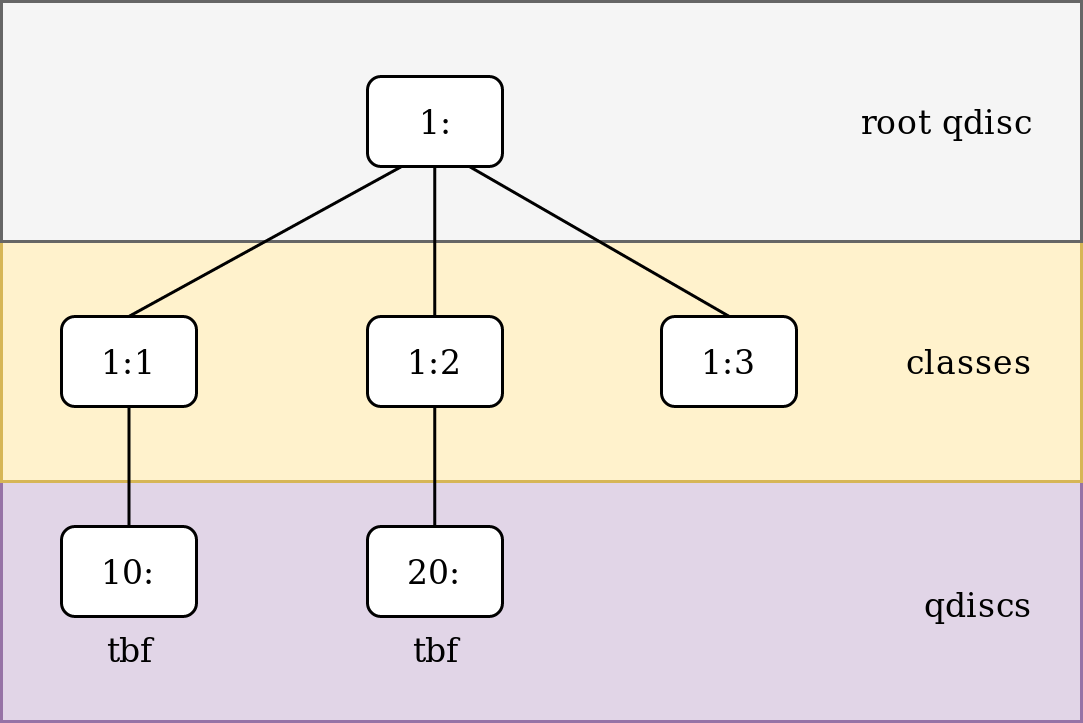
\includegraphics[width=15cm]{figuras/qdiscSingularity.png}}
\caption{Esquema QoS da rede mediante {\tt tc} en contedores Singularity}
\label{qdiscSingularity}
\end{figure}

Unha vez acadado o proceso a seguir para establecer as limitacións externas da rede segundo unha diferenciación mediante usuarios, realizouse a proba pertinente. Desplegáronse dúas máquinas virtuais sobre o Cloud do CESGA correndo Ubuntu Xenial 16.04. Sobre unha destas máquinas aplicáronse as regras dadas no código do apéndice \ref{scriptQoSSingularity} e instalouse a tecnoloxía de contedorización Singularity. Aplicadas as limitacións pertinentes, efectuouse unha conexión SFTP cara a segunda máquina virtual despregada, e procedeuse á transferencia dun arquivo de 5MB, coa que foi posíbel visualizar o correcto establecemento dos límites. O esquema da estrutura despregada pode ser observado na figura \ref{DiagramaQoSRedeSingularity}.\\

\begin{figure}
\centerline{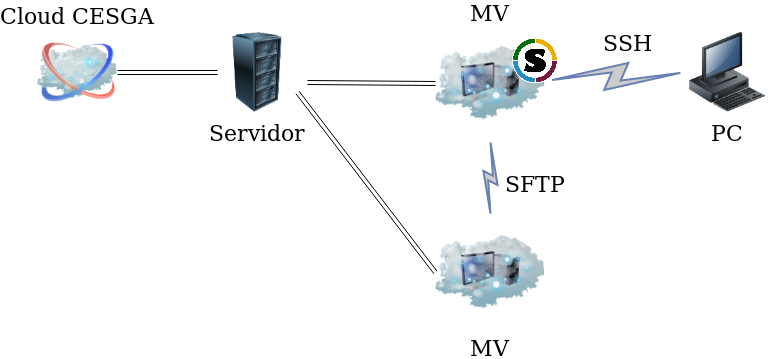
\includegraphics[width=15cm]{figuras/DiagramaQoSRedeSingularity.png}}
\caption{Estrutura do despregue QoS da rede con contedores Singularity}
\label{DiagramaQoSRedeSingularity}
\end{figure}

A proba da transferencia realizouse como superusuario, o cal non tiña nengunha restrición e como \textit{user1}, o cal sí posuía un límite dado. Relizada a proba, as diferenzas e limitacións quedaron demostradas.

\begin{lstlisting}[,caption={Envío SFTP como superusurio}]
root@localhost:/home# singularity shell ubuntu_latest.img 
Singularity: Invoking an interactive shell within container...

Singularity ubuntu_latest.img:/home> sftp user2@10.38.3.5
user2@10.38.3.5's password: 
Connected to 10.38.3.5.
sftp> put photo.jpg 
Uploading photo.jpg to /home/user2/photo.jpg
photo.jpg                                100% 5082KB   5.0MB/s   00:00    
\end{lstlisting}

\begin{lstlisting}[,caption={Envío SFTP como \textit{user1}}]
user1@localhost:/home$ singularity shell ubuntu_latest.img
Singularity: Invoking an interactive shell within container...

Singularity ubuntu_latest.img:/home> sftp user2@10.38.3.5
user2@10.38.3.5's password: 
Connected to 10.38.3.5.
sftp> put photo.jpg 
Uploading photo.jpg to /home/user2/photo.jpg
photo.jpg                                100% 5082KB   3.9KB/s   21:38
\end{lstlisting}

Como pódese apreciar, a transferencia efectuada como superusuario realizouse coa maior celeridade posíbel, enviándose de forma practicamente instantánea. Porén, cando repetimos o envío como o usuario \textit{user1}, pódese ver como as limitacións entran en xogo e esta tarda numerosos minutos en completarse, presentando unha taxa de transferencia incluso menor á indicada.

\subsection{Docker}

O modelo de rede de Docker no seu funcionamento por defecto, é dicir en modo \textit{bridge}, crea unha interface de rede que é empregada para realizar a conexión entre os contedores e a propia máquina. Aproveitaremos o feito de que Docker permite a creación de diferentes interfaces de rede para a conexión dun ou múltiples contedores para aplicar regras de limitación do tráfico de rede, posto que non é posible aplicalo segundo o usuario como no caso de Singularity, xa que os contedores Docker serán executados sempre como superusuario.\\

Novamente, realizouse unha proba de concepto na que se limitou a velocidade do tráfico da rede. Esta vez aplicouse unha limitación mediante unha disciplina de colas sen facer uso de clases, simplificando así o proceso seguido con Singularity. Dita simplificación vén dada porque Singularity non crea un modelado de rede novo, e con esta proba os conceptos deberían quedar claros. Concretamente, aplicouse unha disciplina {\tt tbf} (\textit{Token Bucket Filter}), unha das disciplinas sen clases máis empregadas para limitar o tráfico de rede dunha interface, como é o noso caso. Desta volta estableceuse unha cola de 1024 kbits, permitindo refachos de ata 200 kbits. Os pasos seguidos para establecer estas limitacións poden ser observados no apéndice \ref{scriptQoSDocker}.\\

Para a execución desta proba empregáronse as mesmas máquinas virtuais que no caso anterior, pero agora lanzando un contedor Docker, e aplicando unhas limitacións distintas con {\tt tc}. Novamente, tratouse de enviar un arquivo a outra máquina virtual empregando o protocolo SFTP. O esquema seguido pode ser observado na figura \ref{DiagramaQoSRedeDocker}.\\

\begin{figure}
\centerline{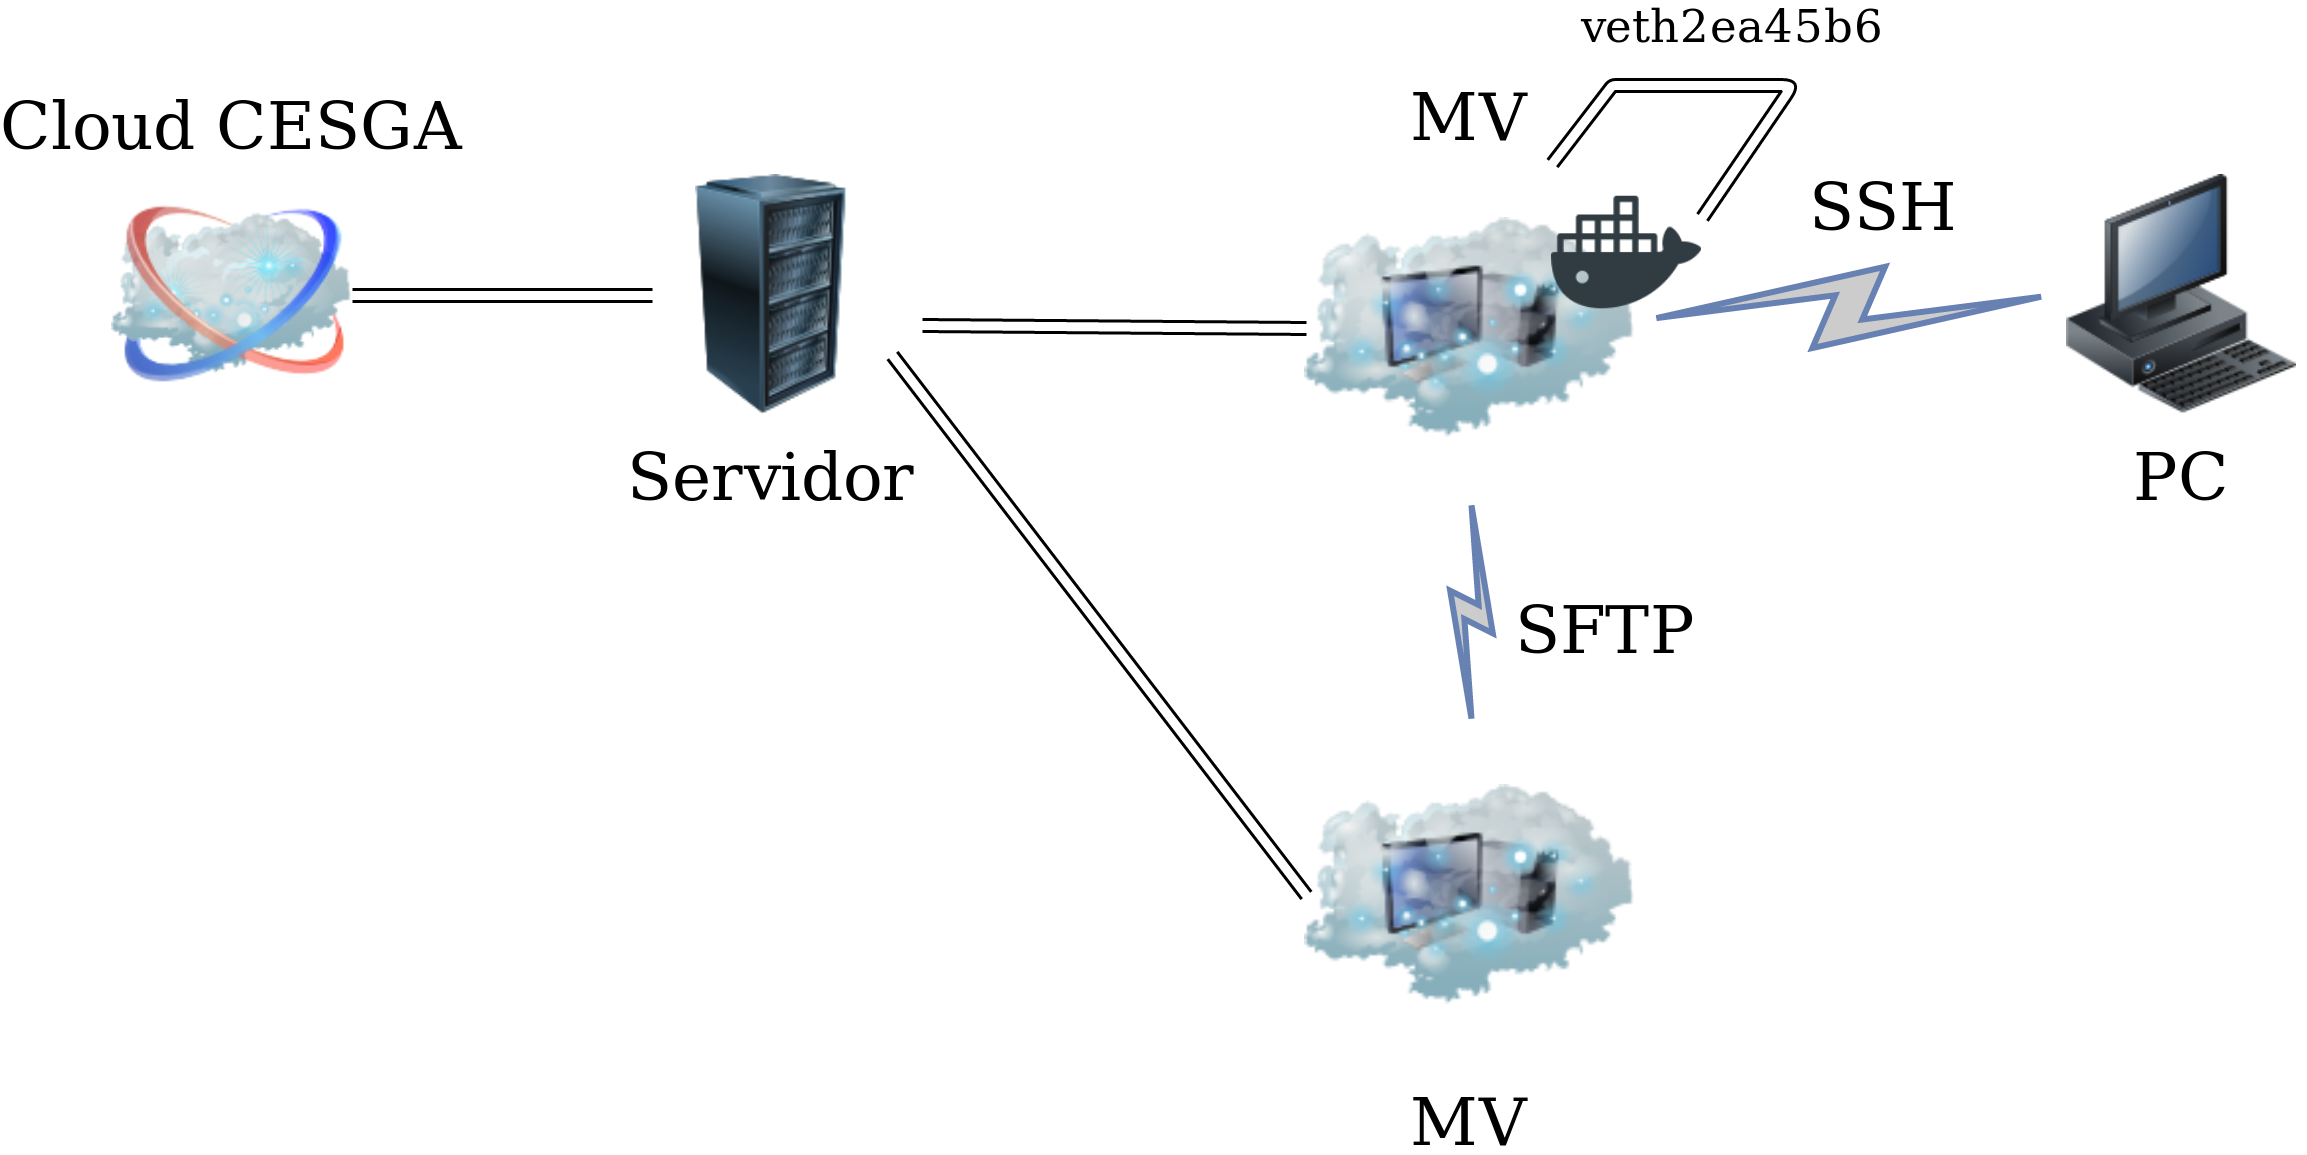
\includegraphics[width=15cm]{figuras/DiagramaQoSRedeDocker.png}}
\caption{Estrutura do despregue QoS da rede con contedores Docker}
\label{DiagramaQoSRedeDocker}
\end{figure}

Para a realización da proba, efectuouse o envío do arquivo nun primeiro intre sen limitación algunha e logo con limitacións sobre a interface de rede do contedor empregado.\\

\begin{lstlisting}[,caption={Envío SFTP sen limitacións}]
sftp> put photo.jpg 
Uploading photo.jpg to /home/user1/photo.jpg
photo.jpg                                100% 6109KB   6.0MB/s   00:00 
\end{lstlisting}

\begin{lstlisting}[,caption={Envío SFTP con limitacións sobre o interface \textit{bridge} de Docker}]
sftp> put photo.jpg
Uploading photo.jpg to /home/user1/photo.jpg
photo.jpg                               15%  960KB   0.0KB/s - stalled -
\end{lstlisting}

Realizadas as probas pódese ver como, unha vez aplicadas as limitacións de rede, o tráfico saínte excede o máximo permitido e a transferencia non pode ser, por tanto, completada.

\section{Cuotas de disco}
\label{quotas}

Para evitar que un contedor empregue a totalidade ou meirande parte do disco, impedindo a correcta execución doutros, cómpre aplicar políticas de limitación no uso do mesmo. Estas políticas poden ser aplicadas doadamente coa emprega de cuotas, permitindo establecer diversidade de límites en función dos usuarios do sistema.\\

Grazas a este feito, os contedores Singularity quedarán perfectamente limitados no referente á utilización do disco. Pola súa contra, os contedores Docker, posto que son executados como superusuario, non se verán limitados, xa que o superusuario terá a capacidade {\tt CAP\_SYS\_RESOURCE}\footnote{http://man7.org/linux/man-pages/man7/capabilities.7.html} activada, a cal permite ignorar os límites de cuotas de disco, entre outras cousas.\\

Para comprobar este feito, realizouse unha proba de concepto dentro dunha máquina virtual Ubuntu Xenial 16.04, na que se estableceron cuotas de disco para un determinado usuario e posteriormente tentouse escribir un ficheiro que superase as limitacións establecidas, facendo uso de contedores baseados en Alpine Linux 3.7.0 (que presentan a característica de que o seu sistema base está deseñado para ocupar só 4-5MB , excluíndo o kernel). As limitacións escollidas foron de 10MB \textit{soft} e de 100MB \textit{hard}. O proceso de aplicación destas cuotas pode ser consultado no apéndice \ref{scriptQuotas}.

\begin{lstlisting}[,caption={Escritura en disco excedendo cuota máxima en contedor Singularity}]
dd if=/dev/zero of=fichero bs=200M count=1
dd: error writing 'fichero': Disk quota exceeded
1+0 records in
0+0 records out
102354944 bytes (102 MB, 98 MiB) copied, 0.701354 s, 146 MB/s
\end{lstlisting}

\begin{lstlisting}[,caption={Escritura en disco excedendo cuota máxima en contedor Docker}]
nuevousuariocuotas@localhost:~$ docker run -ti alpine
/home # dd if=/dev/zero of=fichero bs=200M count=1
1+0 records in
1+0 records out

#Saimos do contedor
nuevousuariocuotas@localhost:~$ docker ps -s 
CONTAINER ID        IMAGE               COMMAND             CREATED             STATUS              PORTS               NAMES               SIZE
1aba32e99ce5        alpine              "/bin/sh"           4 minutes ago       Up 3 seconds                            gifted_bohr         210MB (virtual 214MB)
\end{lstlisting}

Como pódese ver, as cuotas entran en xogo no caso dos contedores Singularity, impedindo a escritura de ficheiros unha vez o límite máximo é excedido. No caso do contedor executado baixo a tecnoloxía de Docker, a escritura é posíbel e os límites son superados. Se ao rematar comprobamos o tamaño actual do contedor, pódese ver coma ocupa un total de 210MB, superando así a cuota total de disco establecida para o usuario.

\subsection{Alternativa en Docker}

A execución de cuotas sobre contedores Docker non resulta efectiva. De todos xeitos, esta tecnoloxía presenta unha xestión sobre os discos máis avanzada, que debe ser estudada con maior detemento.\\

Docker amósanos a posibilidade de almacenar datos no disco dende dúas perspectivas ben diferenciadas:

\begin{enumerate}
    \item Almacenamento persistente no disco: os datos non se perden unha vez remata a execución do contedor.
    \item Almacenamento volátil: os datos soamente son accesíbeis namentres o contedor está executándose.
\end{enumerate}

Para facer esta diferenciación de tipos de almacenamento, Docker presenta varios tipos de montaxe do disco, tal e como pode ser observado na figura \ref{typesOfMountsDocker}. Unha vez dentro do contedor, os datos veranse da mesma forma, no entanto é importante diferencialos para facer un uso adecuado do disco. Así, distinguimos:

\begin{figure}
\centerline{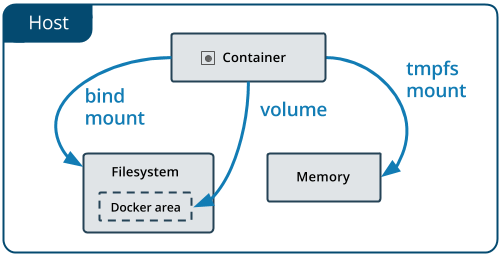
\includegraphics[width=15cm]{figuras/typesOfMountsDocker.png}}
\caption{Tipos de montaxe de disco en Docker. ``\textit{Docker types of mounts}''. Recuperado de https://docs.docker.com/storage/}
\label{typesOfMountsDocker}
\end{figure}

\begin{enumerate}
    \item \textbf{Volumes}: almacenados nalgunha parte do sistema de ficheiros que será xestionado por Docker. Os procesos non pertencentes a Docker non deberían modificar o seu contido, e é considerada a mellor forma de realizar un almacenamento persistente empregando contedores Docker, xa que posúen a característica de estar illados da propia máquina anfitrioa. Ademais, un mesmo volume pode ser compartido entre varios contedores e son doadamente transportábeis cara outra máquina. O seu tamaño pode ser xestionado mediante comandos propios de Docker, pondo solución así a posíbeis ataques de denegación de servizo.
    \item \textbf{\textit{Bind mounts}}: son a outra forma de almacenamento persistente xestionada por Docker. O seu funcionamento baséase na emprega dun espazo de disco compartido coa propia máquina anfitrioa (polo que procesos externos poderían modificar estes datos). Un efecto secundario de este feito é que é posíbel facer cambios no sistema de ficheiros da máquina anfitrioa con permisos de superusuario, puidendo chegar a modificar ou eliminar datos importantes do sistema. Polo tanto, esta forma de almacenamento ten importantes implicacións de seguridade, incluindo un posíbel impacto nos procesos do sistema non referentes a Docker.
    \item \textbf{Montaxes {\tt tmpfs}}: Supoñen a forma de almacenamento non persistente, gardando os datos soamente de forma temporal no tempo de vida do contedor e non chegando a escribir no sistema de ficheiros da máquina anfitrioa. Polo tanto, a emprega deste tipo de montaxes pode ser moi interesante se estamos a facer uso de contedores para despregamentos rápidos e lixeiros, coma podería ser un contedor para probas.
    
    Este tipo de almacenamento presenta a perigosa característica, dende o punto de vista da seguridade informática, de que por defecto non pusúe ningún tipo de limitación no espazo que certo contedor poida empregar. En troques, sí que é posíbel restrinxir o espazo máximo a empregar, coa limitación de que soamente é factíbel baixo a emprega de certos controladores. Docker admite varios controladores de almacenamento, empregando unha arquitectura conectábel, sendo estes os encargados de como as imaxes e os contedores son almacenados e xestionados polo \textit{host}.
    
    Así, se queremos limitar o espazo, deberemos empregar controladores concretos como pode ser \textit{devicemapper}, un framework baseado no kernel de GNU/Linux que sustenta moitas das tecnoloxías avanzadas de xestión de volumes neste tipo de sistemas. Debe ser tido en conta que é precisa unha configuración específica para poder empregar este controlador con Docker que non é admitida por todos os sistemas operativos, polo que o seu uso non resulta trivial. Como dato de interese, destacar que \textit{devicempper} opera a nivel de bloque, no canto de nivel de arquivo, acadando así un rendemento mellor que coa emprega dun sistema de ficheiros a nivel de sistema operativo.
    
    Para comprender un pouco mellor a complexidade asociada, é preciso entender que a elección dun controlador de disco vén limitado por unha complexa matriz de dependencias coma poden ser a edición de Docker, o sistema operativo e mesmamente a distribución do mesmo. Tamén poden ser requeridos paquetes extras para a súa instalación. Ademais, algúns controladores precisan dun formato específico do sistema de ficheiros da máquina anfitrioa, polo que de existir requerimentos externos que limiten a elección dun sistema de ficheiros específico, isto podería limitar enormemente as nosas opcións. Deste xeito, amósase unha táboa de configuracións consideradas estábeis nas versións máis recentes dalgúns dos sistemas operativos GNU/Linux máis soados:

% \usepackage{graphicx}
\begin{table}[H]
\centering
\caption{Táboa de configuracións de controladores de almacenamento}
\label{conf-controladores-almacenamento}
\resizebox{\textwidth}{!}{%
\begin{tabular}{|c|c|}
\hline
\textbf{Distribución GNU/Linux} & \textbf{Controladores de almacenamento recomendados}\\ \hline
Ubuntu & \textit{aufs}, \textit{devicemapper}, \textit{overlay2}, \textit{overlay}, \textit{zfs}, \textit{vfs}\\ \hline
Debian & \textit{aufs}, \textit{devicemapper}, \textit{overlay2}, \textit{overlay}, \textit{vfs}\\ \hline
CentOS & \textit{devicemapper}, \textit{vfs}\\ \hline
Fedora & \textit{devicemapper}, \textit{overlay2} (experimental), \textit{overlay} (experimental), \textit{vfs}\\ \hline
\end{tabular}%
}
\end{table}
    
    Ademais, debemos ter en conta que cada controlador terá algunha vantaxe característica sobre os outros, dependendo da configuración propia de cada sistema. Aínda así, estes aspectos quedan fóra do ámbito do estudo da seguridade, polo que non serán estudados con detemento.
    
    Finalmente, é de vital importancia destacar que se é preciso realizar un cambio nos controladores, os contedores que empregaran o controlador anterior, deixarán de ser accesíbeis, sendo preciso realizar unha parada nos mesmos, exportalos a un medio externo e volver a montalos baixo os novos controladores, o que podería supor unha gran desaceleración do sistema. Polo tanto, é relevante realizar unha adecuada elección do controlador.
    
\end{enumerate}

{\LARGE TODO: proba dos controladores sobre Docker no propio FT2.}\\

{\LARGE TODO: redacción das proba dos controladores sobre Docker en MV Ubuntu.}
